% =====================================================================
%  Appendix: supporting measurements for the Gaussian experiments
%  Place AFTER \section{Conclusion} and BEFORE \begin{thebibliography},
%  preceded by \appendix
% =====================================================================

\section{Supporting Measurements for the Gaussian Experiments}
\label{app:experiments}

\subsection{The regression weight and the velocity field}
\label{app:weighting}

Section \ref{sec:gaussclaims} regresses the velocity field
$\boldsymbol{u}(\xib^{\boldsymbol{x}}_t,t)$ of \eqref{continuousvelocity} in place
of the $\mathcal{L}^2$ best-estimate $\boldsymbol{Y}^{\boldsymbol{x}}_t$. The two
objectives differ by the weight $(T-t)^{-2}$, and both are minimised at the same
function; what follows measures what the weight is worth at finite capacity.

Two networks were trained identically, one against
$\boldsymbol{Y}^{\boldsymbol{x}}_t$ and one against $\boldsymbol{u}$, and then
evaluated as estimators of $\boldsymbol{Y}^{\boldsymbol{x}}_t$ along a common
trajectory, the $\boldsymbol{\sigma}=\boldsymbol{0}$ interpolant, so that neither
is advantaged by seeing its own training noise. The velocity-trained output is
converted by $\xib^{\boldsymbol{x}}_t + (T-t)\,\hat{\boldsymbol{u}}$. Measurement
uses $2048$ triples $(\boldsymbol{x},\boldsymbol{y},t)$ drawn from held-out data.

\begin{table}[htbp]
\begin{center}
\caption{CIFAR-10. Squared error of the endpoint estimate (left) and the same
quantity expressed in the units of the velocity field \eqref{eq:velocityrepeat}
(right). The three networks agree to three decimal places over the first eighty
per cent of the bridge.}
\label{tab:weighting}
\vskip 0.1in
\begin{tabular}{lccccccc}
\toprule
& \multicolumn{3}{c}{endpoint squared error} & & \multicolumn{3}{c}{velocity squared error}\\
\cmidrule{2-4}\cmidrule{6-8}
$t/T$ & $\gamma{=}0.05$ & $\gamma{=}0.3162$ & velocity & & $\gamma{=}0.05$ & $\gamma{=}0.3162$ & velocity\\
\midrule
$0.050$ & $0.20779$ & $0.20783$ & $0.20801$ & & $0.230$ & $0.230$ & $0.230$\\
$0.400$ & $0.04515$ & $0.04534$ & $0.04407$ & & $0.125$ & $0.126$ & $0.122$\\
$0.600$ & $0.02017$ & $0.02051$ & $0.01932$ & & $0.126$ & $0.128$ & $0.121$\\
$0.800$ & $0.00659$ & $0.00698$ & $0.00616$ & & $0.165$ & $0.175$ & $0.154$\\
$0.900$ & $0.00242$ & $0.00275$ & $0.00216$ & & $0.242$ & $0.275$ & $0.216$\\
$0.950$ & $0.00094$ & $0.00120$ & $0.00076$ & & $0.377$ & $0.480$ & $0.305$\\
$0.980$ & $0.00033$ & $0.00052$ & $0.00018$ & & $0.827$ & $1.288$ & $0.455$\\
$0.995$ & $0.00018$ & $0.00028$ & $0.00002$ & & $7.171$ & $11.148$ & $0.698$\\
\bottomrule
\end{tabular}
\end{center}
\end{table}

\begin{figure}[htbp]
\begin{center}
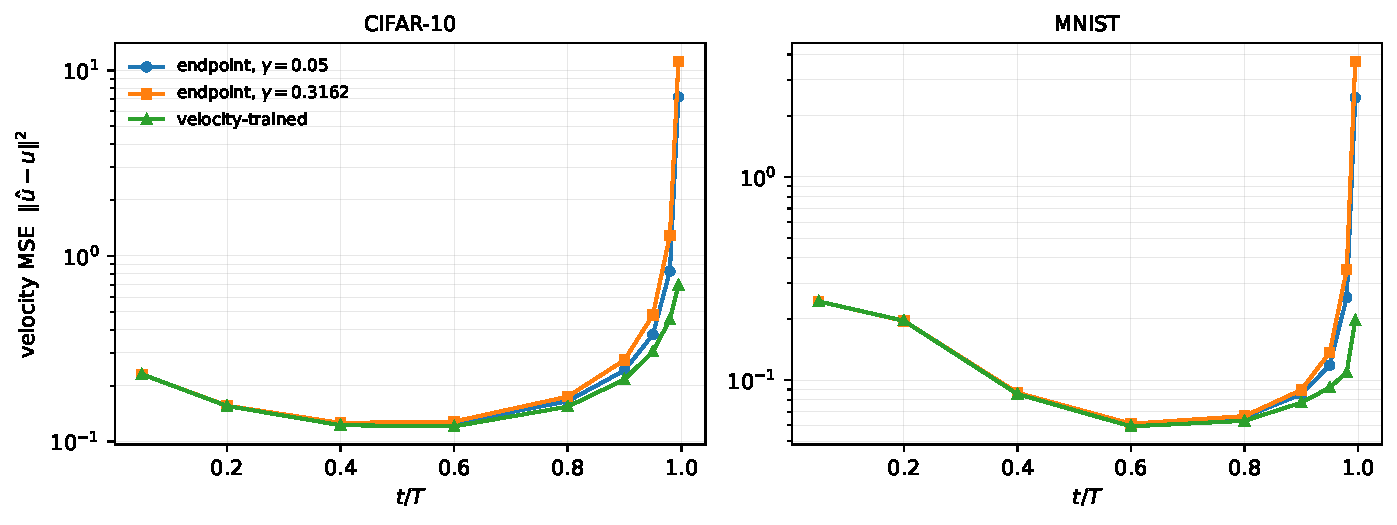
\includegraphics[width=\textwidth]{figures/velocity_error.pdf}
\caption{Squared error of the velocity field along the bridge, logarithmic
vertical scale, $2048$ samples per point on a common
$\boldsymbol{\sigma}=\boldsymbol{0}$ trajectory. Left: CIFAR-10. Right: MNIST.
The curves are indistinguishable until $t\approx0.8\,T$ and separate thereafter.}
\label{fig:velocityerror}
\end{center}
\end{figure}

On CIFAR-10 the correction moves FID at fifty network evaluations from $38.93$ to
$23.23$ at $\boldsymbol{\gamma}=0.3162\,\boldsymbol{I}$, holding architecture,
budget, sampler and evaluation code fixed; both entries are Euler--Maruyama at
$n=2000$. The same asymmetry is present on MNIST and is
marginally larger by the endpoint ratio, $12.4$ against CIFAR-10's $10.3$ at
$t=0.995\,T$, yet in velocity units the MNIST terminal error is $3.70$ against
CIFAR-10's $11.15$: near-binary digits settle their coarse structure well before
$t=0.8\,T$, whereas CIFAR-10 texture is resolved in the terminal region.

The second term of \eqref{eq:velocitytarget} carries conditional variance
$\boldsymbol{\sigma}^2 t/(T-t)$, so larger $\boldsymbol{\gamma}$ purchases its
stochasticity with gradient variance concentrated near the terminal time. The
effect is visible during training, the $\boldsymbol{\gamma}=0.3162$ objective
settling at $0.330$ against $0.190$ for $\boldsymbol{\gamma}=0.05$, and does not
reach FID at the noise levels tested, $23.23$ against $23.34$ at fifty
evaluations.

\clearpage
\subsection{Fidelity, coverage and an alternative feature space}
\label{app:coverage}

\begin{table}[htbp]
\begin{center}
\caption{CIFAR-10 at $n=10\,000$. Precision is the fraction of generated samples
inside the real manifold and recall the fraction of real samples inside the
generated one; coverage is the outlier-robust form of recall. The Kernel
Inception Distance (KID) orders the rows identically to FID at every evaluation
count.}
\label{tab:coverage}
\vskip 0.1in
\resizebox{\textwidth}{!}{%
\begin{tabular}{llcccccc}
\toprule
Model & Simulation & Evals & FID & precision & recall & coverage & KID\\
\midrule
Random-bridge, velocity   & Euler--Maruyama   & $10$ & $\mathbf{20.87}$ & $0.606$ & $\mathbf{0.530}$ & $0.571$ & $\mathbf{0.01391}$\\
Flow Matching             & Euler             & $10$ & $21.21$ & $0.576$ & $0.514$ & $0.565$ & $0.01873$\\
Improved denoising        & ancestral         & $10$ & $27.69$ & $\mathbf{0.617}$ & $0.490$ & $\mathbf{0.578}$ & $0.01827$\\
Improved denoising        & DDIM              & $10$ & $35.69$ & $0.514$ & $0.570$ & $0.396$ & $0.01945$\\
Simple denoising          & ancestral         & $10$ & $52.97$ & $0.472$ & $0.286$ & $0.340$ & $0.05150$\\
Random-bridge, endpoint   & exact posterior   & $10$ & $44.44$ & $0.494$ & $0.365$ & $0.340$ & $0.04809$\\
\midrule
Random-bridge, velocity   & Euler--Maruyama   & $50$ & $11.86$ & $0.614$ & $0.579$ & $0.638$ & $0.00647$\\
Flow Matching             & Euler             & $50$ & $12.45$ & $0.618$ & $0.577$ & $0.670$ & $0.00949$\\
Improved denoising        & ancestral         & $50$ & $\mathbf{8.02}$ & $\mathbf{0.655}$ & $\mathbf{0.583}$ & $\mathbf{0.753}$ & $\mathbf{0.00283}$\\
Improved denoising        & DDIM              & $50$ & $14.82$ & $0.599$ & $0.608$ & $0.636$ & $0.00954$\\
Simple denoising          & ancestral         & $50$ & $20.84$ & $0.581$ & $0.496$ & $0.570$ & $0.01797$\\
Random-bridge, endpoint   & exact posterior   & $50$ & $31.33$ & $0.563$ & $0.458$ & $0.423$ & $0.02989$\\
\midrule
Random-bridge, velocity   & Euler--Maruyama   & $200$ & $10.84$ & $0.607$ & $0.584$ & $0.680$ & $0.00596$\\
Flow Matching             & Euler             & $200$ & $10.88$ & $0.624$ & $0.594$ & $0.680$ & $0.00662$\\
Improved denoising        & ancestral         & $200$ & $\mathbf{7.35}$ & $\mathbf{0.662}$ & $0.602$ & $\mathbf{0.757}$ & $\mathbf{0.00299}$\\
Improved denoising        & DDIM              & $200$ & $10.85$ & $0.619$ & $\mathbf{0.615}$ & $0.682$ & $0.00642$\\
Simple denoising          & ancestral         & $200$ & $13.73$ & $0.622$ & $0.557$ & $0.656$ & $0.01111$\\
Random-bridge, endpoint   & exact posterior   & $200$ & $29.50$ & $0.563$ & $0.448$ & $0.428$ & $0.02650$\\
\bottomrule
\end{tabular}}
\end{center}
\end{table}

The deterministic DDIM sampler at ten evaluations illustrates what the separate
measures reveal: recall of $0.570$ with coverage of $0.396$ indicates a
generated manifold dispersed widely enough to contain real points while few real
points have a generated neighbour nearby. FID reports $35.69$ without
distinguishing this failure from any other.

\begin{table}[htbp]
\begin{center}
\caption{MNIST, $50\,000$ generated samples, scored in the feature space of a
convolutional classifier trained on the MNIST training split. Mode TV is the
total-variation distance between the classifier's predicted-label histogram over
generated samples and the histogram of the data. The final row scores the real
test split against the training split and therefore carries the genuine
train/test difference, not a floor.}
\label{tab:cfid}
\vskip 0.1in
\begin{tabular}{llcccc}
\toprule
Model & Simulation & Evals & classifier FID & mode TV & least-served digit\\
\midrule
Random-bridge      & Euler--Maruyama & $10$ & $\mathbf{27.05}$ & $0.0464$ & $1$ at $0.819$\\
Flow Matching      & Euler           & $10$ & $31.72$ & $\mathbf{0.0438}$ & $0$ at $0.857$\\
Improved denoising & ancestral       & $10$ & $39.64$ & $0.0885$ & $1$ at $0.629$\\
\midrule
Random-bridge      & Euler--Maruyama & $100$ & $\mathbf{0.85}$ & $0.0128$ & $7$ at $0.922$\\
Flow Matching      & Euler           & $100$ & $1.19$ & $0.0147$ & $7$ at $0.923$\\
Improved denoising & ancestral       & $100$ & $1.11$ & $\mathbf{0.0110}$ & $2$ at $0.950$\\
\midrule
Real test split    & ---             & ---   & $1.78$ & $0.0080$ & $6$ at $0.960$\\
\bottomrule
\end{tabular}
\end{center}
\end{table}

At ten evaluations improved denoising diffusion serves the digit $1$ at $62.9$
per cent of its frequency in the data and carries twice the label distortion of
the other two constructs, which is the same ordering as the recall measured on
CIFAR-10 in Table \ref{tab:coverage}.

\clearpage
\subsection{Sensitivity to the diffusion scale and to the simulation scheme}
\label{app:gamma}

\begin{figure}[htbp]
\begin{center}
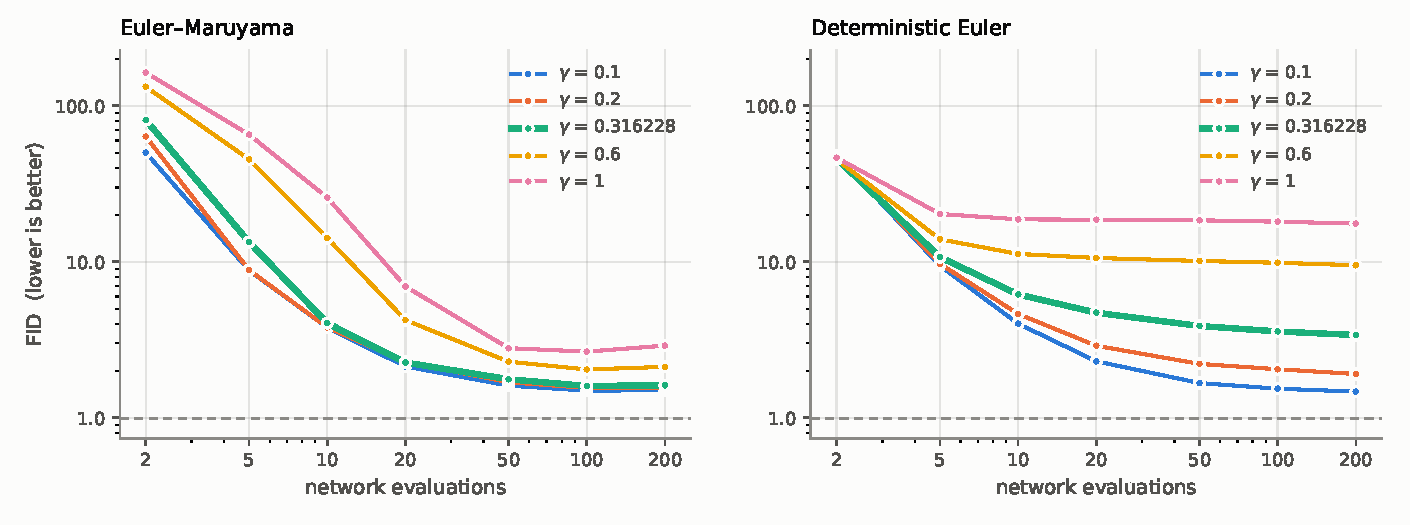
\includegraphics[width=\textwidth]{figures/gamma_sweep.pdf}
\caption{FID against network evaluations for five values of
$\boldsymbol{\gamma}=\boldsymbol{\sigma}\sqrt{T}$ on MNIST, each a separately
trained model sharing architecture, budget and evaluation code; $n=10\,000$,
measured floor $0.70$. Left: the Euler--Maruyama scheme of Algorithm
\ref{alg:simulation}. Right: the deterministic map obtained by deleting the
driving increment.}
\label{fig:gamma}
\end{center}
\end{figure}

Deleting the driving increment $\dd\boldsymbol{Z}_t$ from Algorithm
\ref{alg:simulation} does not yield a valid deterministic simulation of the same
marginals: a deterministic scheme preserving them must follow the probability-flow
ODE, whose drift carries the additional term
$-\tfrac{1}{2}\boldsymbol{\sigma}^2\nabla\log p_t$. The resulting bias is visible
in Figure \ref{fig:gamma} and grows with $\boldsymbol{\gamma}$: at two hundred
evaluations the deterministic map attains $1.47$, $1.91$, $3.39$, $9.51$ and
$17.58$ for $\boldsymbol{\gamma} = 0.1, 0.2, 0.3162, 0.6, 1.0$, while
Euler--Maruyama remains between $1.50$ and $2.90$ across the same range.

On a one-dimensional problem where $\boldsymbol{Y}^{\boldsymbol{x}}_t$ is
available in closed form, so that all residual error is attributable to the
simulation scheme, the Euler--Maruyama and exact-transition schemes both reach
the Monte-Carlo floor in $1$-Wasserstein distance, $0.0095$ and $0.0096$ against
a floor of $0.0091$, while the deterministic map stalls at $0.0625$, with a
terminal standard deviation of $1.726$ against $1.758$. The residual scales with
$\boldsymbol{\gamma}$ as the omitted term predicts: $1.2$ times the floor at
$\boldsymbol{\gamma}=0.0316$, $1.5$ at $0.1$, $6.9$ at $0.3162$ and $18.6$ at
$0.6$.

Smaller $\boldsymbol{\gamma}$ improves both schemes at every evaluation count
above five. On CIFAR-10 under the velocity objective, $\boldsymbol{\gamma}=0.05$
and $\boldsymbol{\gamma}=0.3162$ attain $23.34$ and $23.23$ at fifty
evaluations, a difference within the resolution of that measurement.

\clearpage
\subsection{The conditional variance process against Proposition \ref{propconditionalvarianceprocess}}
\label{app:variance}

Proposition \ref{propconditionalvarianceprocess} states that
$\{\boldsymbol{V}^{\boldsymbol{x}}_t\}$ is a supermartingale under the Loewner
order and Remark \ref{remarkconditionalvarianceprocess} that it vanishes at the
terminal time. The training objective estimates the quantity without additional
computation, since
$\E\|\boldsymbol{y}-f(\xib^{\boldsymbol{x}}_t,t;\boldsymbol{\Theta})\|^2
\to \mathrm{Tr}\,\boldsymbol{V}^{\boldsymbol{x}}_t / n$ once $f$ attains the
$\mathcal{L}^2$ projection, so a trained network measures the process.

Two values are predicted exactly. As $t\to T$ the state determines
$\boldsymbol{Y}$ and the trace must vanish: the measured value is
$9\times10^{-5}$. At $t=0$ the state $\xib^{\boldsymbol{x}}_0=\boldsymbol{x}$ is
independent of $\boldsymbol{Y}$ under the product coupling, so the trace must
equal the mean per-pixel variance of $\boldsymbol{\Psi}$: theory gives $0.21201$
and measurement gives $0.21346$, a ratio of $1.007$. The profile decreases across
all $21$ sampled times (Figure \ref{fig:variance}).

\begin{figure}[htbp]
\begin{center}
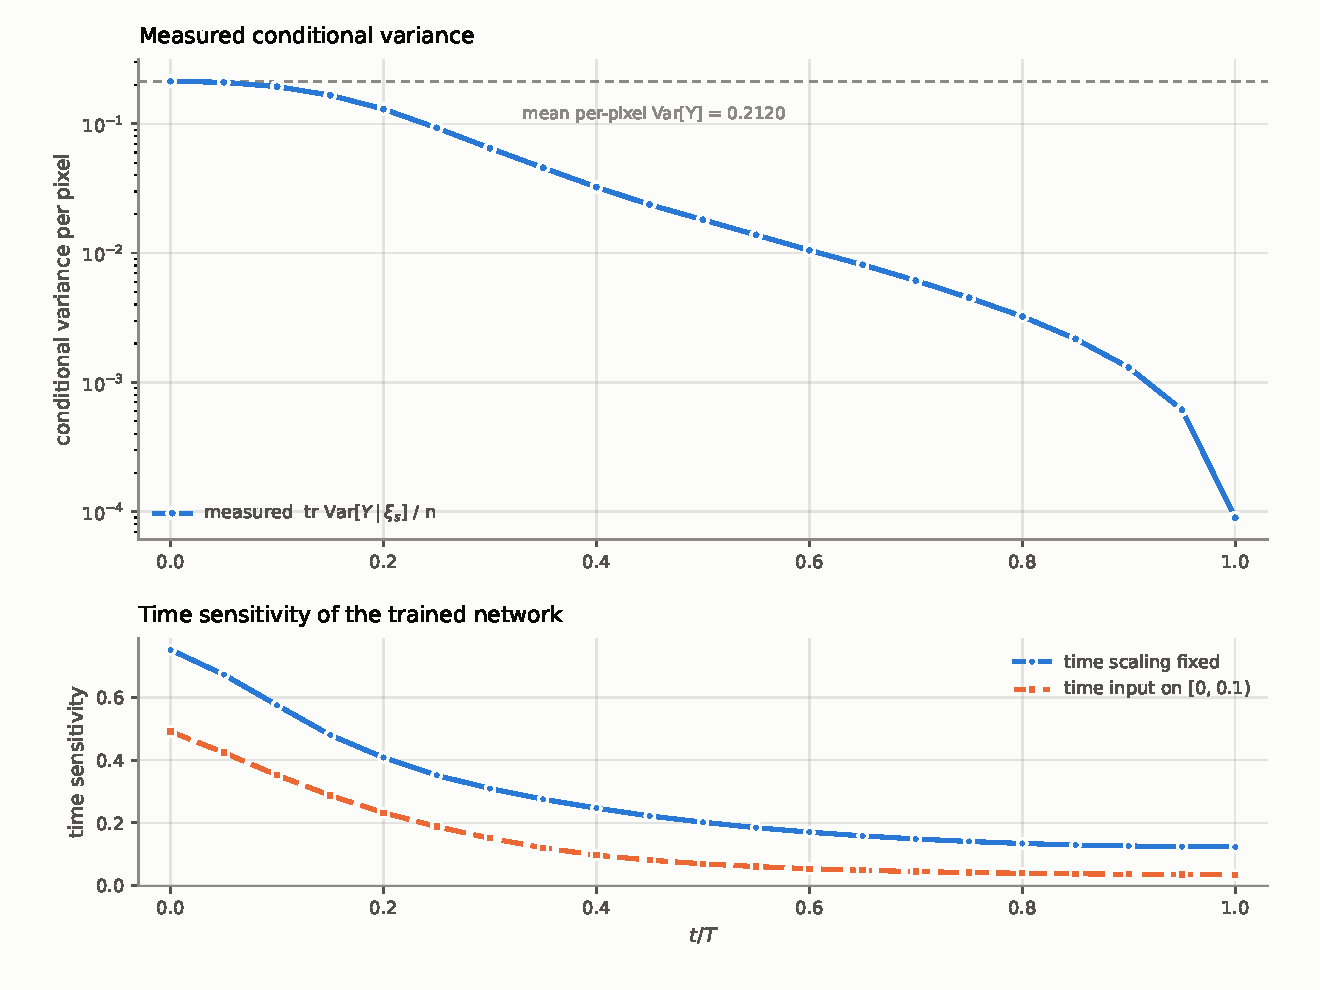
\includegraphics[width=\textwidth]{figures/conditional_variance.pdf}
\caption{Upper panel: $\mathrm{Tr}\,\boldsymbol{V}^{\boldsymbol{x}}_t/n$
estimated by the regression loss of a trained network on held-out data. The
dashed rule marks the mean per-pixel variance of $\boldsymbol{\Psi}$, the value
Proposition \ref{propconditionalvarianceprocess} requires at $t=0$. Lower panel:
the dependence of the network output on its time argument, obtained by holding
the state fixed and sweeping $t$, normalised by the output's own pixel standard
deviation.}
\label{fig:variance}
\end{center}
\end{figure}

A consequence of the same identity is visible in the one-evaluation column of
Table \ref{tab:cifar}. With a single step the conditional expectation map
\eqref{condflowmatch} returns $\E[\boldsymbol{Y}]$ for every initial state, so
all generated samples coincide; the measured FID is $385.98$, and in the
one-dimensional study the terminal standard deviation is $1.6\times10^{-16}$.

Algorithm \ref{alg:simulation} integrates \eqref{nonanticipativerepGMRB} and is
unaffected by this degeneracy at finer grids. The exact-transition scheme of
Proposition \ref{propBrownianBridgeGaussian}, by contrast, replaces the posterior
$\pi_t(\dd\boldsymbol{y})$ by a point mass at its mean, and the law of total
variance shows that this discards
$\left(\tfrac{t'-t}{T-t}\right)^{2}\boldsymbol{V}^{\boldsymbol{x}}_t$ from the
transition variance over $[t,t']$. Restoring an isotropic estimate of that term,
read off the profile of Figure \ref{fig:variance}, raises the coverage of the
exact-transition scheme from $0.602$ to $0.639$ at fifty evaluations, against
$0.638$ for Euler--Maruyama, and lowers its FID from $17.70$ to $14.28$, while
leaving Euler--Maruyama unchanged to four decimal places, as the identity
requires.

\clearpage
\subsection{Generated samples}
\label{app:samples}

\begin{figure}[htbp]
\begin{center}
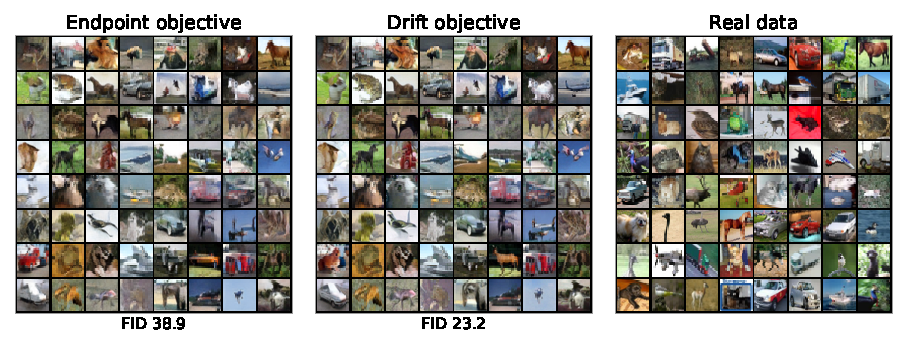
\includegraphics[width=\textwidth]{figures/samples_objective.pdf}
\caption{CIFAR-10 at fifty network evaluations with
$\boldsymbol{\sigma}=\boldsymbol{I}$, $T=0.1$, under the two regression targets
at matched architecture, optimiser, sampler and budget. Both panels are
Euler--Maruyama and both figures are quoted at $n=2000$, the sample count at
which both were measured. The velocity-trained
panel resolves object boundaries and surface texture left diffuse by the
endpoint-trained panel, which is the terminal region of the bridge that the
uniform weight discounts.}
\label{fig:samplesobjective}
\end{center}
\end{figure}

\begin{figure}[htbp]
\begin{center}
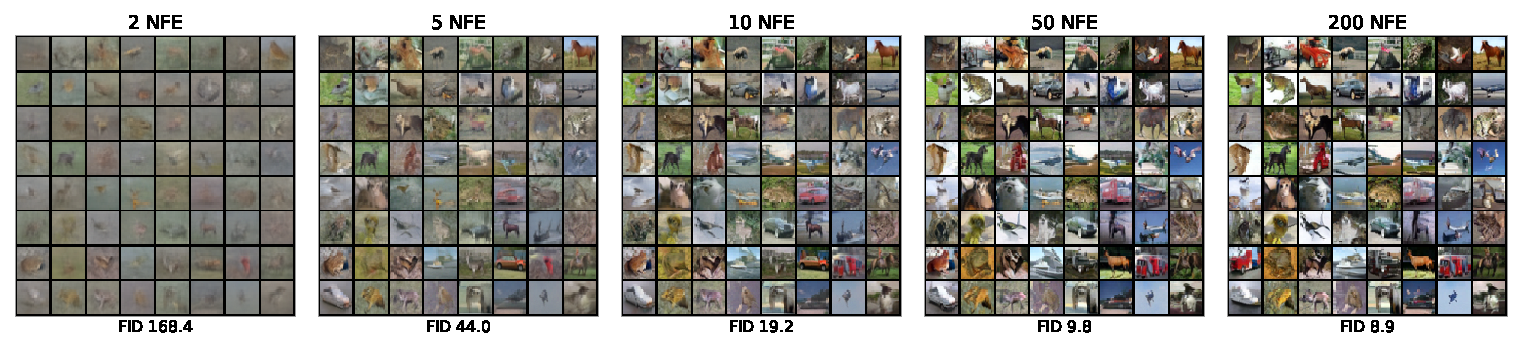
\includegraphics[width=\textwidth]{figures/samples_steps.pdf}
\caption{CIFAR-10 samples against simulation budget,
$\boldsymbol{\sigma}=\boldsymbol{I}$, $T=0.1$, Euler--Maruyama, FID at
$n=50\,000$. Two evaluations return the conditional mean of the data; five
resolve object layout; ten give recognisable objects.}
\label{fig:samplessteps}
\end{center}
\end{figure}

\clearpage

\begin{figure}[htbp]
\begin{center}
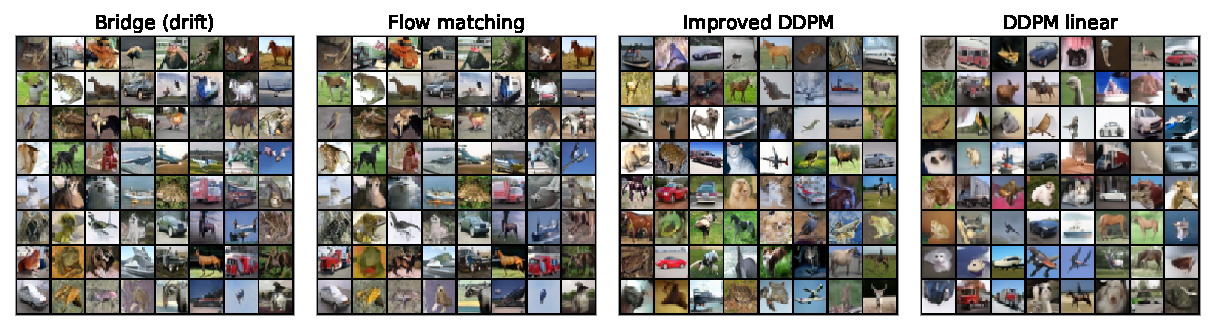
\includegraphics[width=\textwidth]{figures/samples_models.pdf}
\caption{CIFAR-10 at fifty network evaluations under one architecture and one
training budget. Optimisation is AdamW throughout; the random-bridge panel uses
zero weight decay and the three baselines AdamW's default $10^{-2}$.}
\label{fig:samplesmodels}
\end{center}
\end{figure}

\clearpage

\begin{figure}[htbp]
\begin{center}
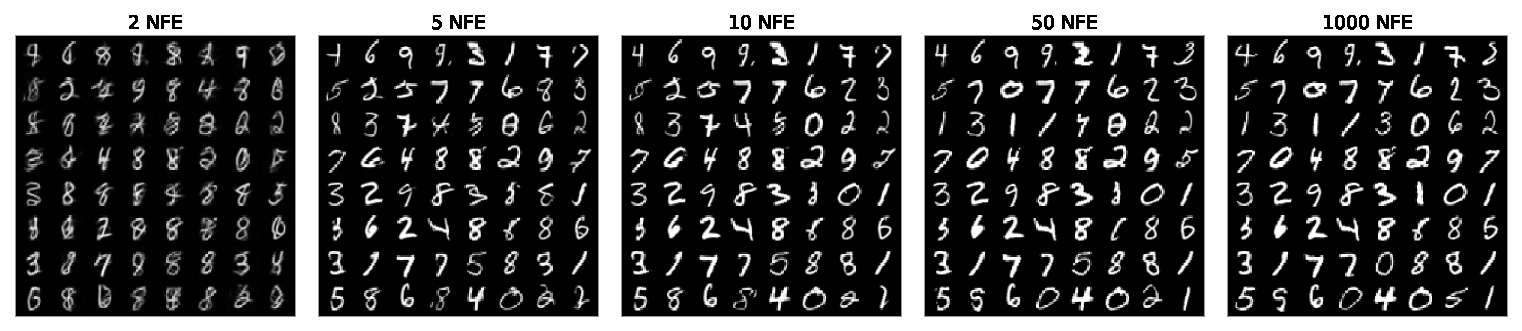
\includegraphics[width=\textwidth]{figures/samples_mnist.pdf}
\caption{MNIST samples against simulation budget,
$\boldsymbol{\sigma}=\boldsymbol{I}$, $T=0.1$, Euler--Maruyama.}
\label{fig:samplesmnist}
\end{center}
\end{figure}

Each panel shows the first $64$ samples of the run named. Initial states are
drawn from one seeded generator in fixed batch order, so the first $64$ are the
same draws regardless of the sample count used for the corresponding FID entry.

% Flush every outstanding float before control returns to the
% main file, so that none can migrate into the bibliography.
\clearpage
